% Created 2011-09-28 Wed 14:44
\documentclass[bigger]{beamer}
\usepackage[utf8]{inputenc}
\usepackage[T1]{fontenc}
\usepackage{fixltx2e}
\usepackage{graphicx}
\usepackage{longtable}
\usepackage{float}
\usepackage{wrapfig}
\usepackage{soul}
\usepackage{textcomp}
\usepackage{marvosym}
\usepackage{wasysym}
\usepackage{latexsym}
\usepackage{amssymb}
\usepackage{hyperref}
\tolerance=1000
\usetheme[titlepagelogo=lal-logo]{Binet}
\usepackage{minted}
\usemintedstyle{emacs}
\pgfdeclareimage[height=1.5cm]{lal-logo}{lal-logo-eps-converted-to}
\logo{\pgfuseimage{lal-logo}}
\hypersetup{colorlinks,linkcolor=blue,urlcolor=blue}
\providecommand{\alert}[1]{\textbf{#1}}

\title{D\'eveloppeur \`a l'IN2P3}
\author{S\'ebastien Binet}
\date{2011-09-29}

\institute[LAL]{\insertlogo\hskip0.1cm}
\begin{document}

\maketitle





\section{jdev}
\label{sec-1}
\begin{frame}
\frametitle{Qui suis-je ?}
\label{sec-1-1}


\begin{itemize}
\item \alert{2008-\ldots{}:} Post-doc au LAL (Orsay)
\begin{itemize}
\item d\'eveloppeur sur le cadriciel \verb~ATHENA~ d'ATLAS
\item d\'eveloppeur d'outils logiciels pour les analyses de physique
\item \emph{R\&D} multi-c\oe urs
\end{itemize}
\item \alert{2005-2008:} Post-doc \`a LBL (Berkeley)
\begin{itemize}
\item d\'eveloppeur sur le cadriciel \verb~ATHENA~ d'ATLAS
\item d\'eveloppeur d'outils pour les analyses de physique
\item d\'eveloppement d'outils logiciels pour le suivi des performances
\item \emph{R\&D} multi-c\oe urs
\end{itemize}
\item \alert{2002-2005:} Doctorant au LPC (Clermont-Fd)
\begin{itemize}
\item analyse de physique aupr\`es du d\'etecteur ATLAS
\item d\'eveloppement d'outils logiciels pour la physique
\end{itemize}
\end{itemize}
\end{frame}
\begin{frame}
\frametitle{Structure d'accueil}
\label{sec-1-2}


Laboratoire de l'Acc\'el\'erateur Lin\'eaire.

\begin{itemize}
\item Unit\'e Mixte de Recherche IN2P3/CNRS - Paris-Sud (UMR 8607)
\item Centr\'e sur la Physique des Particules
\item + forte composante en Cosmologie et Astrophysique
\item Mission de transmission des connaissances
\begin{itemize}
\item \emph{via} l'enseignement
\item \emph{via} la communication
\end{itemize}
\item Services techniques et administratifs
\item Services de conception et r\'ealisation en m\'ecanique et
  \'electronique
\item Services technologies de l'information
\item Programme de \emph{R\&D} dans le domaine des acc\'el\'erateurs
\end{itemize}
\end{frame}
\begin{frame}
\frametitle{LAL}
\label{sec-1-3}


\begin{itemize}
\item 352 agents (2011/01/01)
\begin{itemize}
\item 126 chercheurs
\begin{itemize}
\item 49 CNRS
\item 11 enseignants
\item 12 \'em\'erites
\item 20 post-docs \& CDDs
\item 32 doctorants
\item 2 \'etudiants master
\end{itemize}
\item 226 Ing\'enieurs Techniciens
\begin{itemize}
\item 29 CDDs
\item 4 ITARFs
\end{itemize}
\end{itemize}
\end{itemize}
\end{frame}
\begin{frame}
\frametitle{Activit\'e - Contexte}
\label{sec-1-4}


\begin{itemize}
\item d\'eveloppement de logiciel pour la collaboration ATLAS
\item contexte exp\'erimental
\begin{itemize}
\item ATLAS - trigger
\end{itemize}
\item outils
\begin{itemize}
\item savannah
\item lxr (Linux Cross Referencer)
\item NICOS (NIghtly COntrol System)
\item ATN (Atlas Testing Nightly)
\item RTT (RunTime Tester)
\item FCT (Full Chain Test)
\item CMT (Configuration Management Tool)
\item WLCG (Worldwide LHC Computing Grid)
\item pacman (package manager)
\item RPM
\item SVN, CVS (->2009)
\end{itemize}
\end{itemize}
\end{frame}
\begin{frame}
\frametitle{Illustration}
\label{sec-1-5}


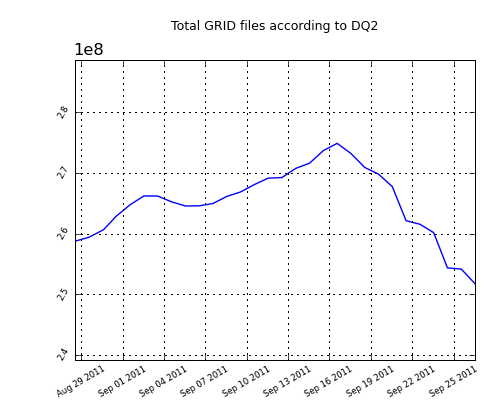
\includegraphics[width=.9\linewidth]{figs/global_evolution_files30.png}
\end{frame}

\end{document}
